\chapter{Einführung und Ziele}

\section{Aufgabenstellung und Anforderungen}

Es soll ein verteiltes Steuerungssystem gemäß den Prinzipien verteilter Systeme nach Tanenbaum \& van Steen entworfen und implementiert werden. Über ein ITS-Board (bspw. STM32F4) soll ein autonomer Roboter innerhalb eines kontrollierten Areals (z.B. BT7 R7.65 – als realer Testbereich) sicher und effizient gesteuert werden. Die verteilte Architektur soll dabei explizit gewährleisten, dass durch Fehlverhalten der Software oder Architektur keine Gefahr für anwesende entstehen kann.

\subsection*{Funktionale Beschreibung}


\begin{itemize}
	
	\item \textbf{Betreiber - System}
		\begin{itemize}
			\item Nutzer wählt genau einen Roboterarm aus
			\item Nutzer gibt Steuerbefehl an genau einen Roboterarm
			\item System zeigt an, ob Roboterarm verfügbar
			\item Notstop löst sofortigen Stopp des ausgewählten Roboters aus
		\end{itemize}
		
	\item \textbf{System}
		\begin{itemize}
			\item Roboterarme stoppen, sobald nicht mehr von aussen kontrollierbar
			\item automatisches Erkennen von Hinzufügen und Entfernen von Roboterarmen
			
		\end{itemize}
	
\end{itemize}

\begin{figure}[h!]
	\centering
	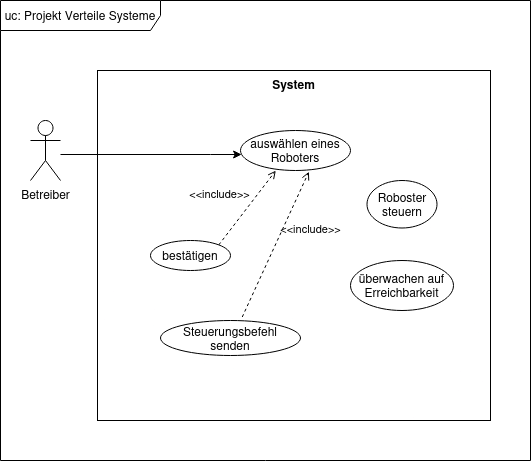
\includegraphics[scale=.5]{diagrams/use_case.png}
	\caption{Funktionales Use Case Diagramm der Aufgabenstellung}
	\label{fig:meine-grafik}
\end{figure}

\newpage
\section{Qualitätsziele}
% Aus VS Skript Kapitel 2.4 Seite 23
% TODO zu jeden Punkt eine Definition oder entfernen
% TODO messbar definieren

Das verteilte Steuerungssystem soll eine Reihe von nicht-funktionalen Anforderungen erfüllen, um einen sicheren, wartbaren und erweiterbaren Betrieb im Einsatzumfeld zu gewährleisten. 

\subsection{Ziele für Software Engineering}
\begin{table}[h!]
    \centering
    \begin{tabular}{p{4cm}|p{5cm}|p{5cm}|}
        \hline
        \textbf{Ziel} & \textbf{Beschreibung} & \textbf{Metrik} \\
        \hline
        Funktionalität &  
        %Der Roboter muss Steuerbefehle korrekt umsetzen, auf Umgebungsdaten reagieren und vordefinierte Aufgaben zuverlässig erfüllen.
        & Alle Abnahmetests werden erfolgreich bestanden
        \\
        \hline
        Zuverlässigkeit & 
        %Teilausfälle dürfen den Gesamtsystembetrieb nicht gefährden. Fehlererkennung und -toleranz müssen integriert sein.
        & Das System ist über dem gesamten Abnahmezeitraum stabil (ca. 1,5 h)
        \\
        \hline
        Skalierbarkeit & 
        Zusätzliche Roboter oder Komponenten sollen ohne Änderungen an der bestehenden Architektur integrierbar sein. 
        & Es können beliebig viele Roboter hinzugefügt und entfernt werden (0 - N)
        \\
        \hline
        Leistung & 
        %Reaktionszeiten auf Steuerbefehle und Ereignisse müssen innerhalb definierter Zeitgrenzen liegen. 
        & Reaktionszeit max. 250 ms
        \\
        \hline
        Sicherheit (Safety) & 
        Es bewegt sich immer genau ein Roboterarm. Sollte das System nicht wie gewünscht reagieren, wird ein sicherer Zustand erreicht
        %Das System darf unter keinen Umständen eine Gefährdung für Personen/Gegenstände darstellen. Bei Fehlern muss sofort ein sicherer Zustand erreicht werden (z.B. Notstopp). 
        & Reaktionszeit max. 250 ms, bis Roboterarm stoppt
        \\
        %\hline
        %Wartbarkeit & 
        %Der Code muss modular, gut dokumentiert und testbar sein. Fehlerdiagnose und Protokollierung sollen integriert sein. 
        %& 
        %\\
        \hline
        %Portabilität & %Die Software soll ohne großen Aufwand auf vergleichbaren Embedded-Systemen lauffähig sein. 
        %& nicht relevant
        %\\
        %\hline
        Benutzerfreundlichkeit & %Konfiguration und Überwachung müssen intuitiv bedienbar und gut visualisiert sein. 
        & Keine Einweisung erforderlich
        \\
        \hline
        Anpassbarkeit & 
        %Neue Funktionen, Sensoren oder Regeln sollen ohne tiefgreifende Änderungen am System integrierbar sein. 
        & 
        \\
        \hline
        Kompatibilität & 
        %Das System soll mit bestehenden Standards und Protokollen kommunizieren können. 
        & 
        \\
        \hline
    \end{tabular}
    \caption{Qualitätsziele der Software Engineering}
    \label{tab:seziele}
\end{table}

\clearpage
\subsection{Ziele der Verteilte Systeme}
    \begin{table}[h!]
        \centering
        \begin{tabular}{p{4cm}|p{5cm}|p{5cm}|}
            \hline
            \textbf{Ziel} & \textbf{Beschreibung} & \textbf{Metrik} \\
            \hline
            Ressourcenteilung  & ...& \\
            Offenheit & ...& \\
            Skalierbarkeit & ...& siehe Tabelle \ref{tab:skalierbarkeit} \\
            Verteilung Transparenz & ...& siehe Tabelle \ref{tab:transparenzen} \\
            \hline
        \end{tabular}
        \caption{Qualitätsziele der Verteilten Systeme}
        \label{tab:vsziele}
    \end{table}
    
\subsubsection{Skalierbarkeit}
    \begin{table}[h!]
            \centering
            \begin{tabular}{p{4cm}|p{5cm}|p{5cm}|}
                \hline
                \textbf{Ziel} & \textbf{Metrik} & \textbf{Metrik} \\
                \hline
                Vertikale Skalierung   & ... &\\
                \hline
                Horizontale Skalierung & ...& \\
                \hline
                Räumliche Skalierbarkeit &  & 1 \\
                \hline
                Funktionale Skalierbarkeit & ... & \\
                \hline
                Administrative-Skalierbarkeit & &1 \\
                \hline
            \end{tabular}
            \caption{Skalierbarkeit von verteilten Systemen}
            \label{tab:skalierbarkeit}
        \end{table}
    
\newpage
\subsubsection{Verteilungs-Transparenzen}
    \begin{table}[h!]
            \centering
            \begin{tabular}{p{4cm}|p{5cm}|p{5cm}|}
                \hline
                \textbf{Ziel} & \textbf{Beschreibung} & \textbf{Metrik} \\
                \hline
                Zugriffstransparenz   & ...&\\
                \hline
                Lokalitäts-Transparenz  & ...&\\
                \hline
                Migrationstransparenz & ...&\\
                \hline
                Replikationstransparenz &...&\\
                \hline
                Fehlertransparenz &... &\\
                \hline
                Ortstransparenz & .. &\\
                \hline
                Skalierbarkeits-Transparenz & ... & \\
                %Concurrency
                %Relocation
                \hline
            \end{tabular}
            \caption{Verteilungs-Transparenzen}
            \label{tab:transparenzen}
        \end{table}
        



\clearpage
\section{Stakeholder}
Die folgenden Gruppen sind direkt oder indirekt vom System betroffen:

\begin{itemize}
    \item \textbf{Endnutzer:} Personen, die mit dem Roboter interagieren (z.B. Lehrpersonal, Kinder im Testbereich)
    \item \textbf{Entwicklerteam:} Zuständig für Entwurf, Umsetzung, Tests und Wartung des Systems
    \item \textbf{Betreiber:} Verantwortlich für die Überwachung und den sicheren Betrieb des Systems im realen Umfeld
    \item \textbf{Professor:} Person, die für die Bewertung des Systems verantwortlich ist und Rahmenbedingungen vorgibt.

\end{itemize}



